% \iffalse meta-comment
%
% ledarab.dtx
% Author: Peter Wilson (Herries Press) herries dot press at earthlink dot net
% Copyright 2005 Peter R. Wilson
%
% This work may be distributed and/or modified under the
% conditions of the LaTeX Project Public License, either
% version 1.3 of this license or (at your option) any 
% later version.
% The latest version of the license is in
%    http://www.latex-project.org/lppl.txt
% and version 1.3 or later is part of all distributions of
% LaTeX version 2003/06/01 or later.
%
% This work has the LPPL maintenance status "author-maintained".
%
% This work consists of the files listed in the README file.
%
%
%<*driver>
\documentclass[twoside]{ltxdoc}
\usepackage{url}
  \usepackage[draft=false,
              plainpages=false,
              pdfpagelabels,
              bookmarksnumbered,
%              hyperindex=true
              hyperindex=false
             ]{hyperref}
\providecommand{\phantomsection}{} % just in case hyperref is not used
\usepackage{graphicx}
% a simpler version of chngpage.sty's adjustwidth environment
\newenvironment{addtomargins}[2]{%
  \begin{list}{}{%
  \topsep 0pt
  \addtolength{\leftmargin}{#1}%
  \addtolength{\rightmargin}{#2}%
  \listparindent \parindent
  \itemindent \parindent
  \parsep \parskip
  }%
  \item[]}{\end{list}}
\makeatletter
  \@mparswitchfalse
\makeatother
\EnableCrossrefs
\CodelineIndex
%%\OnlyDescription
\renewcommand{\MakeUppercase}[1]{#1}
\pagestyle{headings}
\setcounter{StandardModuleDepth}{1}
\setcounter{IndexColumns}{2}
\begin{document}
  \raggedbottom
  \DocInput{ledarab.dtx}
\end{document}
%</driver>
%
% \fi
%
% \CheckSum{821}
%
% \makeatletter
% \newcommand*{\DescribeIt}{\leavevmode\@bsphack\begingroup\MakePrivateLetters
%  \Describe@It}
% \newcommand*{\Describe@It}[1]{\endgroup
%   \marginpar{\raggedleft\PrintDescribeEnv{#1}}%
%   \SpecialItIndex{#1}\@esphack\ignorespaces}
% \newcommand*{\SpecialItIndex}[1]{\@bsphack
%   \index{#1\actualchar{\protect\ttfamily#1}\encapchar usage}\@esphack}
%     
% \DoNotIndex{\@,\@@par,\@beginparpenalty,\@empty}
% \DoNotIndex{\@flushglue,\@input}
% \DoNotIndex{\@makefnmark,\@makeother,\@maketitle}
% \DoNotIndex{\@namedef,\@ne,\@spaces,\@tempa}
% \DoNotIndex{\@tempb,\@tempswafalse,\@tempswatrue}
% \DoNotIndex{\@thanks,\@thefnmark,\@topnum}
% \DoNotIndex{\@@,\@elt,\@forloop,\@fortmp,\@gtempa,\@totalleftmargin}
% \DoNotIndex{\",\/,\@ifundefined,\@nil,\@verbatim,\@vobeyspaces}
% \DoNotIndex{\|,\~,\ ,\active,\advance,\aftergroup,\begingroup,\bgroup}
% \DoNotIndex{\mathcal,\csname,\def,\documentstyle,\dospecials,\edef}
% \DoNotIndex{\egroup}
% \DoNotIndex{\else,\endcsname,\endgroup,\endinput,\endtrivlist}
% \DoNotIndex{\expandafter,\fi,\fnsymbol,\futurelet,\gdef,\global}
% \DoNotIndex{\hbox,\hss,\if,\if@inlabel,\if@tempswa,\if@twocolumn}
% \DoNotIndex{\ifcase}
% \DoNotIndex{\ifcat,\iffalse,\ifx,\ignorespaces,\index,\input,\item}
% \DoNotIndex{\jobname,\kern,\leavevmode,\leftskip,\let,\llap,\lower}
% \DoNotIndex{\m@ne,\next,\newpage,\nobreak,\noexpand,\nonfrenchspacing}
% \DoNotIndex{\obeylines,\or,\protect,\raggedleft,\rightskip,\rm,\sc}
% \DoNotIndex{\setbox,\setcounter,\small,\space,\string,\strut}
% \DoNotIndex{\strutbox}
% \DoNotIndex{\thefootnote,\thispagestyle,\topmargin,\trivlist,\tt}
% \DoNotIndex{\twocolumn,\typeout,\vss,\vtop,\xdef,\z@}
% \DoNotIndex{\,,\@bsphack,\@esphack,\@noligs,\@vobeyspaces,\@xverbatim}
% \DoNotIndex{\`,\catcode,\end,\escapechar,\frenchspacing,\glossary}
% \DoNotIndex{\hangindent,\hfil,\hfill,\hskip,\hspace,\ht,\it,\langle}
% \DoNotIndex{\leaders,\long,\makelabel,\marginpar,\markboth,\mathcode}
% \DoNotIndex{\mathsurround,\mbox,\newcount,\newdimen,\newskip}
% \DoNotIndex{\nopagebreak}
% \DoNotIndex{\parfillskip,\parindent,\parskip,\penalty,\raise,\rangle}
% \DoNotIndex{\section,\setlength,\TeX,\topsep,\underline,\unskip,\verb}
% \DoNotIndex{\vskip,\vspace,\widetilde,\\,\%,\@date,\@defpar}
% \DoNotIndex{\[,\{,\},\]}
% \DoNotIndex{\count@,\ifnum,\loop,\today,\uppercase,\uccode}
% \DoNotIndex{\baselineskip,\begin,\tw@}
% \DoNotIndex{\a,\b,\c,\d,\e,\f,\g,\h,\i,\j,\k,\l,\m,\n,\o,\p,\q}
% \DoNotIndex{\r,\s,\t,\u,\v,\w,\x,\y,\z,\A,\B,\C,\D,\E,\F,\G,\H}
% \DoNotIndex{\I,\J,\K,\L,\M,\N,\O,\P,\Q,\R,\S,\T,\U,\V,\W,\X,\Y,\Z}
% \DoNotIndex{\1,\2,\3,\4,\5,\6,\7,\8,\9,\0}
% \DoNotIndex{\!,\#,\$,\&,\',\(,\),\+,\.,\:,\;,\<,\=,\>,\?,\_}
% \DoNotIndex{\discretionary,\immediate,\makeatletter,\makeatother}
% \DoNotIndex{\meaning,\newenvironment,\par,\relax,\renewenvironment}
% \DoNotIndex{\repeat,\scriptsize,\selectfont,\the,\undefined}
% \DoNotIndex{\arabic,\do,\makeindex,\null,\number,\show,\write,\@ehc}
% \DoNotIndex{\@author,\@ehc,\@ifstar,\@sanitize,\@title,\everypar}
% \DoNotIndex{\if@minipage,\if@restonecol,\ifeof,\ifmmode}
% \DoNotIndex{\lccode,\newtoks,\onecolumn,\openin,\p@,\SelfDocumenting}
% \DoNotIndex{\settowidth,\@resetonecoltrue,\@resetonecolfalse,\bf}
% \DoNotIndex{\clearpage,\closein,\lowercase,\@inlabelfalse}
% \DoNotIndex{\selectfont,\mathcode,\newmathalphabet,\rmdefault}
% \DoNotIndex{\bfdefault}
% \DoNotIndex{\newcommand}
%
% \newcommand{\dtxfilename}{\texttt{ledarab.dtx}}
% \def\fileversion{v0.1} \def\filedate{2005/03/24}
%
% \changes{v0.1}{2005/03/24}{First public release}
%
% \hyphenation{man-u-script man-u-scripts}
%
% \newcommand{\Lpack}[1]{\textsf{#1}}
% \newcommand{\Lclass}[1]{\textsf{#1}}
% \newcommand{\file}[1]{\texttt{#1}}
% \newcommand{\env}[1]{\texttt{#1}}  ^^A for environment names
% \newcommand{\ledpar}{ledpar}
% \newcommand{\ledmac}{ledmac}
% \newcommand{\Ledmac}{\Lpack{\ledmac}}
% \newcommand{\Ledpar}{\Lpack{\ledpar}}
% \newcommand{\edmac}{\texttt{EDMAC}}
% \newcommand{\tabmac}{\texttt{TABMAC}}
% \newcommand{\edstanza}{\texttt{EDSTANZA}}
% \newcommand{\ArabTeX}{\texttt{ArabTeX}}
% \newcommand{\Larabtex}{\Lpack{arabtex}}
% \newcommand{\Lafoot}{\Lpack{afoot}}
% \newcommand{\Lledarab}{\Lpack{ledarab}}
% \newcommand{\PWcomment}[1]{}
% \newenvironment{PW}{\itshape}{}
% \renewenvironment{PW}{\sffamily}{}
% \newcommand{\texbook}{\textit{TeXbook}}
% \newcommand{\thetexbook}{\textit{The TeXbook}}
%
% ^^A PW added following as the definitions are at some unknown elsewhere
% \newcommand{\egstart}{}
% \newcommand{\egmid}{}
% \newcommand{\egend}{}
%
% \renewcommand{\egstart}{%
%    \par
%    \begingroup
%    \centering
%    \begin{minipage}{0.45\textwidth}}
% \renewcommand{\egmid}{%
%    \end{minipage}\hfill\begin{minipage}{0.45\textwidth}}
% \renewcommand{\egend}{%
%    \end{minipage}\par\endgroup}
%
% \title{Critical editions and arabic typesetting: \\
%       the \Lpack{ledarab} and \Lpack{afoot} packages\thanks{This file (\dtxfilename)
% has version number \fileversion, last revised \filedate.}}
% \author{%
% Peter Wilson \\
% Herries Press\thanks{\texttt{herries dot press at earthlink dot net}}}
%
% \date{}
%
%
% \maketitle
%
%
% \begin{abstract}
% The \Ledmac{} package, which is based on the \PlainTeX\ set of
% \edmac\ macros, has been used for some time for typesetting critical 
% editions, and the \ArabTeX{} system enables the typesetting of arabic
% texts. 
%
% The \Lafoot{} package is an extension to the \Larabtex{} package
% to enable footnotes in arabic texts and the \Lledarab{} package 
% provides an interface between \Larabtex{} and \Ledmac{} (also \Ledpar) 
% for arabic text 
% in critical editions.
% \end{abstract}
%
% \tableofcontents
% \listoffigures
%
%
% \section{Introduction}
%
%    The \edmac{} macros \cite{EDMACTUG} for typesetting critical editions 
% of texts
% have been available for use with TeX for some years, and the 
% \Larabtex{} package \cite{ARABTEX} provides for arabic typesetting. 
% These two
% works are interfaced by the \Lpack{aedpatch} package provided as
% part of the \ArabTeX{} distribution. 
%
% Following the introduction of \edmac{}
% there had been a small but constant demand for a
% version that could be used with LaTeX. The \Ledmac{}
% package \cite{LEDMAC} was introduced in 2003 in an attempt to satisfy 
% that request. This was extended in 2004 by the \Ledpar{} package 
% \cite{LEDPAR} to allow the typesetting of parallel critical texts.
% The \Lledarab{} package provides an interface between the \Larabtex{}
% and the \Ledmac{} (and \Ledpar) packages.
%    The package has to try and coerce \TeX{} into paths it was not designed
% for. Use of the package, therefore, may produce some surprising results.
%
%    I initially used version 3.10 (2001/09/16) of the \Larabtex{} package 
% but when I moved to version 3.11 (2003/08/22) I found that the code
% for footnotes (in \file{afoot.sty}) no longer worked. The \Lafoot{} package
% provided here is based on the obsolete 3.10 version, until a working
% version\footnote{I made queries about this on the \texttt{comp.text.tex} 
% newsgoup on 2005/01/06 but got no responses.} 
% of \file{afoot.sty} is provided in the \ArabTeX{} distribution.
%
% \section{The \Lpack{afoot} package}\label{howto}
%
% The \Larabtex{} package automatically calls the \Lafoot{} package. If you
% want to use my version of \Lafoot{} just make sure that it is found by
% LaTeX before the \ArabTeX's version, for example by having a copy in 
% your working directory.
%
% \DescribeMacro{\footnote}
% The \cs{footnote}\marg{text} produces a numbered footnote. Unlike
% the usual LaTeX \cs{footnote} macro there is no optional argument
% for specifying the number.
%
% \DescribeMacro{\LRfootnotes}
% Inside an \env{arabtext} environment the \cs{LRfootnotes} declaration 
% causes following footnotes to be in normal left to right (LtoR) roman text, 
% left adjusted and with the number at the left.
%
% \DescribeMacro{\RLfootnotes}
% \DescribeMacro{\arabfootnotes}
% Inside an \env{arabtext} environment the \cs{RLfootnotes} or
% \cs{arabfootnotes}  declaration 
% causes any following footnotes to be in right to left (RtoL) arabic script,
% right adjusted and with the number at the right. 
% In normal text the footnotes are normal.
%
% To get an arabic footnote in normal text try: \\
% \verb?...roman\footnote{\RL{arabic}}...? \\
% The footnote will be left adjusted but the note's text will be arabic.
%
%
% \section{The \Lpack{ledarab} package}
%
% The \Lledarab{} package\footnote{I offered an earlier version to Prof.
% Lagally towards the end of 2003 for possible addition to his
% \Larabtex{} package but got no response to my messages.}
% is partially based on Klaus Lagally's \file{aedpatch.sty}
% and lets the \Ledmac{} package's critical apparatus be applied
% to arabic texts. The packages must be used in the following order:
% \begin{verbatim}
%    \usepackage{ledmac}
%    \usepackage{ledpar} % if you need parallel texts.
%    \usepackage{arabtex}
%    \usepackage{ledarab}
% \end{verbatim}
%
%     The package is very limited --- only the basic numbering and 
% critical footnotes are supported. Even then, all critical notes
% are left adjusted with the lemma and note in left to right order, although
% the lemma and/or note may be in RtoL arabic script. Items like familiar 
% footnotes, endnotes, tabulars and so on are left to you the user.
%
% In normal numbered text you can use the \cs{RL} macro within the critical
% aparatus for short pieces of arabic.
% \begin{verbatim}
% \beginnumbering
% \pstart
% Normal \edtext{latin}{\Cfootnote{roman}} text.
% Normal \edtext{\RL{latin}}{\Cfootnote{\RL{roman}}} text.
% ...
% \end{verbatim}
% In the first line above the lemma and footnote will both be in latin 
% script while in the second line they will both be in arabic script; in
% each case, though, the lemma is at the left and the note follows on the 
% right.
%
% \begin{verbatim}
% \beginnumbering
% \pstart
% \begin{arabtext}
% Arabic \edtext{script}{\Afootnote{roman}} text.
% Arabic \edtext{script}{\Afootnote{\LR{roman}}} text.
% Arabic \edtext{script}{\Afootnote{\RL{arabic}}} text.
% Arabic \edtext{\LR{error}}{\Afootnote{roman}} text.
% \end{arabtext}
% \pend
% ...
% \end{verbatim}
% In the first and second lines above the lemma is in arabic script and 
% the note in
% latin script, while in the third line both the lemma and the note
% are in arabic script. Using \cs{LR} as part of the lemma, as in the last  
% line causes errors.
%
% \begin{verbatim}
% \beginnumbering
% \begin{arabtext}
% \pstart
% Arabic \edtext{script}{\Afootnote{messy}} text.
% Arabic \edtext{script}{\Afootnote{\LR{messy}}} text.
% Arabic \edtext{script}{\Afootnote{\RL{arabic}}} text.
% \pend
% \end{arabtext}
% ...
% \end{verbatim}
% In the first two lines above the lemma is in arabic and the note
% is in what looks like (to me at least) arabic, but it is all messed up. 
% In the last line both the lemma and the note are 
% in arabic.
%
% \DescribeMacro{\arablnumrep}
% \DescribeMacro{\restorelnumrep}
% Line numbers are normally typeset in latin script arabic numerals and LtoR.
% Following the \cs{arablnumrep} declaration they will be typeset in
% arabic script numerals and RtoL. The \cs{restorelnumrep} ensures the
% regular line numbers. Use the declarations like:
% \begin{verbatim}
% \arablnumrep
% \begin{arabtex} ... \end{arabtex}
% \restorelnumrep
% \end{verbatim}
%
% \DescribeMacro{\latinarabic}
% \DescribeMacro{\arabiclatin}
% Arabic script naturally has a greater height or leading 
% (larger \cs{baselineskip})
% than latin text. Parallel normal texts and parallel arabic texts align
% naturally, as do parallel columns of latin/arabic or arabic/latin texts.
% However, left to their own devices pages of parallel arabic and 
% normal text will not align.
% 
%    If you are setting normal text on the left pages and arabic script
% on the right using the \cs{latinarabic} declaration should align them. 
% Similarly when you have arabic script on the left and latin script
% on the right use the \cs{arabiclatin} declaration.
%
% \DescribeMacro{\ledarabstrut}
% \DescribeMacro{\savestruts}
% \DescribeMacro{\restorestruts}
% The \cs{ledarabstrut} strut is the height of a line of arabic script
% and is used to increase the height of latin text lines to match
% arabic script lines. The definition is: \\
% \verb?\newcommand*{\ledarabstrut}{\rule[-1ex]{0pt}{4ex}}? \\
% If it does not quit match the arabic script in your case then change the 
% \verb?4ex? appropriately.
%
% The macro \cs{savestruts} saves the current definitions of the struts
% used in the left and right texts (\cs{latinarabic} and \cs{arabiclatin}
% change these). The macro \cs{restorestruts} set the definitions of the
% left and right struts to match those stored by the last \cs{savestruts}.
% The package calls \cs{savestruts} itself to store the default struts.
%
%     For example, with regular text on the left and arabic on the right
% then the general scheme is:
% \begin{verbatim}
% \savestruts
% \begin{pages}
% \begin{Leftside}
%   \beginnumbering
%   \pstart
%     normal text
%     ...
% \end{Leftside}
% \begin{Rightside}
%   \begin{arabtext}
%   \beginnumbering
%   \pstart
%     arabic text
%     ...
% \end{Rightside}
% \latinarabic
% \Pages
% \restorestruts
% \end{pages}
% \end{verbatim}
%
%    In the above, if it had been: \\
% \verb?\begin{arabtext}?\\
% \verb?  \Pages?\\
% \verb?\end{arabtext}?\\
% Then a redefinition of \cs{ledarabstrut} as: \\
% \verb?\renewcommand*{\ledarabstrut}{\rule[-1ex]{0pt}{3.75ex}}? \\
% might provide better alignment of the latin text with the arabic.
%
%     Life gets complicated regarding lemmas and notes when there are 
% parallel latin and arabic texts.
% Consider that there are the following left (latin) and right (arabic) texts
% \begin{verbatim}
% \begin{Leftside}
%  ...
% 1) \edtext{latin}{\Afootnote{roman}}...
% 2) \edtext{\RL{latin}}{\Afootnote{\RL{roman}}}...
% 3) \edtext{\LR{latin}}{\Afootnote{\LR{roman}}}...
% ...
% \end{Leftside}
% \begin{Rightside}
% \begin{arabtext}
% ...
% A) \edtext{script}{\Bfootnote{arabic}}...
% B) \edtext{script}{\Bfootnote{\RL{arabic}}}...
% C) \edtext{script}{\Bfootnote{\LR{arabic}}}...
% ...
% \end{Rightside}
% \end{verbatim}
% and they are to be output as matching pages. If they are output simply as: \\
% \verb?\Pages? \\
% then the lemmas and notes for the marked lines are: \\
% 1) latin lemma, latin note \\
% 2) arabic lemma, arabic note \\
% 3) latin lemma, latin note \\
% A) arabic lemma, latin note \\ 
% B) arabic lemma, arabic note \\ 
% C) arabic lemma, latin note 
%
%    On the otherhand, if they are output via: \\
% \verb?\begin{arabtext} \Pages \end{arabtext}? \\
% then the lemmas and notes for the marked lines are: \\
% 1) latin lemma, messed arabic note \\
% 2) arabic lemma, arabic note \\
% 3) latin lemma, messed arabic note \\
% A) arabic lemma, messed arabic note \\
% B) arabic lemma, arabic note \\ 
% C) arabic lemma, messed arabic note 
%
%
% \StopEventually{%
% ^^A \addcontentsline{toc}{section}{\protect\numberline{B}Index}
% \addcontentsline{toc}{section}{Index}
% \PrintIndex
% ^^A \addtocontents{toc}{\protect\end{multicols}}
% }
%
% \section{The \Lpack{afoot} implementation}
% \label{afootimpl}
%
% The \Lafoot{} package is effectively an extraction from
% the \Lpack{alatex} package of \ArabTeX, v3.10, 2000/05/08.
%
% Announce the name and version of the package, which is 
% targetted for LaTeX2e.
%
%    \begin{macrocode}
%<*afoot>
\NeedsTeXFormat{LaTeX2e}
\ProvidesPackage{afoot}[2005/03/24 v0.1 PW's version of ArabTeX's afoot.sty]

%    \end{macrocode}
%
% The package redefines the internals of the LaTeX \cs{footnote} macro
% along the lines of the \cs{vfootnote} macro in \PlainTeX. It also
% does some things a bit differently if the \Lpack{fnpara} package
% has been used. 
%
% \begin{macro}{\@makefntext}
% I don't know why this is here as it is also defined as part of the
% \cs{@footnotetext} macro below.
%    \begin{macrocode}
\ifx \footglue \undefined % normal case
\else                   % fnpara.sty is present
  \long\def\@makefntext#1{{$^{\@thefnmark}$}#1\nobreak }
\fi

%    \end{macrocode}
% \end{macro}
%
% \begin{macro}{\@footnotetext}
%    \begin{macrocode}
%%% Make the LaTeX \cs{footnote} catcode-safe, like in Plain TeX.

\def \@footnotetext {%        new, do not yet read footnote text
  \insert \footins \bgroup
  \ifx \footglue \undefined %  prepare normal footnote
    \interlinepenalty \interfootnotelinepenalty \floatingpenalty \@MM
    \splittopskip \footnotesep \splitmaxdepth \dp \strutbox
  \else
    \global\long\def \@makefntext ##1{{$^{\@thefnmark }$}##1\nobreak }%
    \setbox0=\hbox \bgroup % fnpara.sty is present
    \floatingpenalty=20000 \footnotesize
  \fi
  \edef\@currentlabel{\csname p@footnote\endcsname\@thefnmark}%
  \a@fntext }

%    \end{macrocode}
% \end{macro}
%
% \begin{macro}{\@mpfootnotetext}
% The version for \env{minpage}s.
%    \begin{macrocode}
\def \@mpfootnotetext {%
  \global \setbox \@mpfootins \vbox \bgroup
    \edef \@currentlabel {\csname p@mpfootnote\endcsname \@thefnmark }%
  \unvbox \@mpfootins \reset@font \a@fntext }

%    \end{macrocode}
% \end{macro}
%
% \begin{macro}{\a@fntext}
% A common portion of the code for the footnote text in both normal and 
% \env{minipage} environments.
%    \begin{macrocode}
\def \a@fntext {% common part for footnote text
  \footnotesize \hsize \columnwidth \@parboxrestore \clubpenalty 5000
  \@makefntext {\rule {\z@ }{\footnotesep }}\futurelet \next \fo@t }

%    \end{macrocode}
% \end{macro}
%
% The next set of macros are from the \cs{vfootnote} macro 
% (\textit{The TeXbook}, Appendix B)
% \begin{macro}{\fo@t}
% Copy from \textit{TeXbook}.
%    \begin{macrocode}
%%%%%%%%%%%%%%%%%%%%%%%% \footnote, parts from Plain %%%%%%%%%%%%%%%%%

\def\fo@t{%
  \ifcat
    \bgroup \noexpand\next 
    \let\next\f@@t
  \else
    \let\next\f@t 
  \fi 
  \next }
%    \end{macrocode}
% \end{macro}
%
% \begin{macro}{\f@@t}
% Copy from \textit{TeXbook}.
%    \begin{macrocode}
\def\f@@t{\bgroup\aftergroup\@foot\let\next}
%    \end{macrocode}
% \end{macro}
%
% \begin{macro}{\f@t}
% Copy from \textit{TeXbook}.
%    \begin{macrocode}
\def\f@t#1{#1\@foot}
%    \end{macrocode}
% \end{macro}
%
% \begin{macro}{\@foot}
% This has a bit more to it than the \textit{TeXbook} macro.
%    \begin{macrocode}
\def\@foot{\unskip \strut \lineskiplimit -20pt \endgraf \egroup }

%    \end{macrocode}
% \end{macro}
%
% \begin{macro}{\a@footnote}
% \begin{macro}{\@foot}
% \begin{macro}{\@footnotemark}
% These macros are for normal footnotes from within an arabic environment.
%    \begin{macrocode}
%%%%%%%%% footnote inside an Arabic environment, Roman document style

\def\a@footnote{%
  \def\@foot{% ArabTeX-LaTeX version
    \ifx \footglue \undefined % normal case
      \unskip \strut
    \else                     % fnpara.sty is present
      \penalty-10 \hskip\footglue \egroup % box 0
      \dp0=0pt \ht0=\fudgefactor\wd0 \box0 
     \fi
     \egroup \arab@codes \set@arabfont \test@token }%
  \def\@footnotemark{\af@fnmarkb@x \a@spacetrue}%
  \rmfamily \parindent \a@parindent \unarab@codes \footnote }

%    \end{macrocode}
% \end{macro}
% \end{macro}
% \end{macro}
%
% \begin{macro}{\af@fnmarkb@x}
% This saves some tokens as the code is used in several places.
%    \begin{macrocode}
\def\af@fnmarkb@x{%
  \a@spacefalse \putword@box \@makefnmark}

%    \end{macrocode}
% \end{macro}
%
% \begin{macro}{\a@footnotemark}
% \begin{macro}{\@footnotemark}
% These are also for normal footnotes from within an arabic environment.
%    \begin{macrocode}
\def\a@footnotemark{%
  \def\@footnotemark{\af@fnmarkb@x \a@spacefalse \arab@codes \test@token}%
  \unarab@codes \footnotemark }

%    \end{macrocode}
% \end{macro}
%
% \begin{macro}{\a@@footnote}
% \begin{macro}{\@footnotemark}
% \begin{macro}{\a@fntext}
% These macros are for arabic footnotes from within an arabic environment.
%    \begin{macrocode}
%%%%%%%%% footnote inside an Arabic environment, Arabic document style

\def\a@@footnote{% ArabTeX-LaTeX version
  \def\@footnotemark{\af@fnmarkb@x \a@spacetrue}%
  \def\a@fntext{\a@@fntext }%
  \footnote }

%    \end{macrocode}
% \end{macro}
% \end{macro}
% \end{macro}
%
% \begin{macro}{\a@@fntext}
% This is also for arabic footnotes, being the common portion of the code
% for footnote text in both normal and \env{minipage} texts.
%    \begin{macrocode}
\def\a@@fntext#1{% some common code for footnote text
  \def\end{%
    \a@par \egroup \test@token }%
  \hsize \columnwidth \@parboxrestore
  \initlineb@x \@footnotemark \test@token #1 \end }

%    \end{macrocode}
% \end{macro}
%
% \begin{macro}{\a@@footnotemark}
% \begin{macro}{\@footnotemark}
% As are these.
%    \begin{macrocode}
\def\a@@footnotemark{%
  \def\@footnotemark{\af@fnmarkb@x \a@spacetrue \test@token}%
  \footnotemark }

%    \end{macrocode}
% \end{macro}
% \end{macro}
%
% \begin{macro}{\LRfootnotes}
% Inside an \env{arabtext} environment the \cs{LRfootnotes} declaration 
% results in normal footnotes, left adjusted.
%    \begin{macrocode}
\def \LRfootnotes {% left to right, Arabic document
  \let \a@c@footnote \a@footnote
  \let \a@c@footnotemark \a@footnotemark }
\all@wcmd \LRfootnotes

%    \end{macrocode}
% \end{macro}
%
% \begin{macro}{\RLfootnotes}
% Inside an \env{arabtext} environment the \cs{RLfootnotes} declaration 
% results in arabic footnotes, right adjusted. In normal text the footnotes
% are normal.
%    \begin{macrocode}
\def \RLfootnotes {% right to left, Arabic document
  \let \a@c@footnote \a@@footnote
  \let \a@c@footnotemark \a@@footnotemark }
\all@wcmd \RLfootnotes
%    \end{macrocode}
% \end{macro}
%
% \begin{macro}{\arabfootnotes}
% \cs{arabfootnotes} is an alias for \cs{RLfootnotes}.
%    \begin{macrocode}
\let \arabfootnotes \RLfootnotes
\all@wcmd \arabfootnotes

%    \end{macrocode}
% \end{macro}
%
% Make \cs{LRfootnotes} the default.
%    \begin{macrocode}
\LRfootnotes

%    \end{macrocode}
%
% The end of the package
%
%    \begin{macrocode}
%</afoot>
%    \end{macrocode}
%
%
% \section{The \Lpack{ledarab} implementation}
% \label{ledarabimpl}
%
% The \Lledarab{} package is based on the original \Lpack{aedpatch}
% from the \ArabTeX{} distribution.
%
% Announce the name and version of the package, which is for LaTeX2e.
%
%    \begin{macrocode}
%<*ledarab>
\NeedsTeXFormat{LaTeX2e}
\ProvidesPackage{ledarab}[2005/03/24 v0.1 Cooperation between arabtex and ledmac]

%    \end{macrocode}
%
% \begin{macro}{\tr@ce@n}
% \begin{macro}{\tr@ce@ff}
% I think, but don't know, that by appropriate (re)definitions of these 
% you can get \Larabtex{}
% to produce some tracing of what is going on, perhaps by setting 
% \cs{tracingmacros} to 1 instead of 0.
%    \begin{macrocode}
\providecommand*{\tr@ce@n}{\tracingmacros 0}
\providecommand*{\tr@ce@ff}{\edef \tr@ce@n 
	{\nxp\tracingmacros \the\tracingmacros }\tracingmacros 0}
\let \tr@ce@n \relax

%    \end{macrocode}
% \end{macro}
% \end{macro}
%
% \begin{macro}{\if@l@dparpack}
% \begin{macro}{\@l@dparpacktrue}
% \begin{macro}{\@l@dparpackfalse}
% We need a flag for knowing if \Ledpar{} is being used.
%    \begin{macrocode}
\newif\if@l@dparpack
  \@l@dparpackfalse
\@ifpackageloaded{ledpar}{\@l@dparpacktrue}{\@l@dparpackfalse}

%    \end{macrocode}
% \end{macro}
% \end{macro}
% \end{macro}
%
% \subsection{Adjusting the baselines}
%
% \begin{macro}{\do@linehook}
% Arabic lines are taller than roman lines, so add some height to 
% numbered lines.
%    \begin{macrocode}
\renewcommand*{\do@linehook}{% 
  \advance\baselineskip 1ex}

%    \end{macrocode}
% \end{macro}
%
%
% \begin{macro}{arabledparfixi}
% If the \Ledpar{} package is loaded we have to change several of its
% macros. We can't do this simply within an \cs{if@l@dparpack} because
% of the internal \cs{if}s. Hence, we define a macro whose expansion
% is the necessary changes.
%
%    \begin{macrocode}
%%%%%%%%%%%%%%%%%%%%% ledpar fix %%%%%%%%%%%%%%%%%%%%%%%%%%%%
\newcommand{\arabledparfixi}{%
%    \end{macrocode}
% \begin{macro}{\do@lineLhook}
% \begin{macro}{\do@lineRhook}
% Increase the height of numbered lines.
%    \begin{macrocode}
\renewcommand*{\do@lineLhook}{% 
  \advance\baselineskip 1ex}
\renewcommand*{\do@lineRhook}{%
  \advance\baselineskip 1ex}
%    \end{macrocode}
% \end{macro}
% \end{macro}
%
% \begin{macro}{\a@l@dparparamsL}
% \begin{macro}{\a@l@dparparamsR}
% Variations on \cs{a@parparams} from \ArabTeX's \file{aoutput.sty}.
% These are required to take account of the differing widths, by setting
% \cs{a@hsize} appropriately.
%    \begin{macrocode}
\newcommand*{\a@l@dparparamsL}{%
  \ifnum \parshape = \z@ 
     \a@hsize \Lcolwidth
     \a@leftmargin \z@
  \else
    \a@hsize \Lcolwidth \a@leftmargin \@totalleftmargin
  \fi
  \a@leftmargin \z@
  \a@prevgraf \z@ \spreadfalse }
\newcommand*{\a@l@dparparamsR}{%
  \ifnum \parshape = \z@ 
     \a@hsize \Rcolwidth
     \a@leftmargin \z@
  \else
    \a@hsize \Rcolwidth \a@leftmargin \@totalleftmargin
  \fi
  \a@leftmargin \z@
  \a@prevgraf \z@ \spreadfalse }
%    \end{macrocode}
% \end{macro}
% \end{macro}
%
% \begin{macro}{\Leftsidehook}
% \begin{macro}{\Rightsidehook}
% 
%    \begin{macrocode}
\renewcommand*{\Leftsidehook}{%
  \let\a@parparams\a@l@dparparamsL}
\renewcommand*{\Rightsidehook}{%
  \let\a@parparams\a@l@dparparamsR}
%    \end{macrocode}
% \end{macro}
% \end{macro}
%
% \begin{macro}{\ledarabstrut}
% \begin{macro}{\ledstrutL}
% \begin{macro}{\ledstrutR}
% \begin{macro}{\savestruts}
% \begin{macro}{\restorestruts}
% \begin{macro}{\latinarabic}
% \begin{macro}{\arabiclatin}
% In order to get parallel arabic and normal texts to line up
% a strut has to be added to each latin line to hide their different heights;
% this is \cs{ledarabstrut}. The commands \cs{savestruts} and 
% \cs{restorestruts} save and restore the original left/right strut 
% definitions. The declaration \cs{latinarabic} is for left and right texts
% being latin and arabic, and for left arabic and right latin use 
% \cs{arabiclatin}.
%    \begin{macrocode}
\newcommand*{\ledarabstrut}{%
  \rule[-1ex]{0pt}{4ex}}
\newcommand*{\savestruts}{%
  \let\oldl@dstr@tL\ledstrutL
  \let\oldl@dstr@tR\ledstrutR}
\newcommand*{\restorestruts}{%
  \let\ledstrutL\oldl@dstr@tL
  \let\ledstrutR\oldl@dstr@tR}
\newcommand*{\latinarabic}{%
  \def\ledstrutL{\ledarabstrut}%
  \def\ledstrutR{}}
\newcommand*{\arabiclatin}{%
  \def\ledstrutL{}%
  \def\ledstrutR{\ledarabstrut}}

%    \end{macrocode}
% \end{macro}
% \end{macro}
% \end{macro}
% \end{macro}
% \end{macro}
% \end{macro}
% \end{macro}
% At last, the end of \cs{arabledparfixi}.
%    \begin{macrocode}
}% end of \newcommand{\arabledparfixi}{...

%    \end{macrocode}
% \end{macro}
%
% Perform the fix for \Ledpar{} if necessary.
%    \begin{macrocode}
\if@l@dparpack
  \arabledparfixi
  \savestruts
\fi
%%%%%%%%%%%%%%%%%%%%% end major ledpar fix %%%%%%%%%%%%%%%%%%%%%%%%%%%%

%    \end{macrocode}
% \end{macro}
%
% \subsection{Lemmas}
%
% \begin{macro}{\a@c@edtext}
% This is the internal version of \cs{edtext}. The parameters
% have their original catcodes.
%    \begin{macrocode}
\newcommand*{\a@c@edtext}{%
  \tr@ce@n \leavea@vmode \unarab@codes 
\begingroup
  \tr@ce@ff \rmfamily \tr@ce@n \a@@edtext}

%    \end{macrocode}
% \end{macro}
%
% \begin{macro}{\a@@edtext}
% An auxiliary routine to kill leading blanks and remove spurious braces 
% from \cs{edtext}'s second argument.
%    \begin{macrocode}
\newcommand*{\a@@edtext}[1]{%
%%%  \def\next@command{\a@@@edtext {\RL{#1}}}% causes errors
  \def\next@command{\a@@@edtext {#1}}% 
  \futurelet \next@token \test@space }

%    \end{macrocode}
% \end{macro}
%
% \begin{macro}{\a@edget@text}
% Get flags and lemma.
%    \begin{macrocode}
\def\a@edget@text #1\@@{%
  \a@edappend{\flag@start}\a@@Linsert{#1}}

%    \end{macrocode}
% \end{macro}
%
% \begin{macro}{\a@edend@lemma}
% Another utility routine.
%    \begin{macrocode}
\newcommand*{\a@edend@lemma}{%
  \ifx\end@lemmas\empty \else
    \gl@p\end@lemmas\to\x@lemma
    \x@lemma
    \global\let\x@lemma=\relax
  \fi}

%    \end{macrocode}
% \end{macro}
%
% \begin{macro}{\a@edput@text}
% Unpack \cs{Linsertb@x}.
%    \begin{macrocode}
\newcommand*{\a@edput@text}{%
  \a@Lunpack \putwordb@x {\ins@skip }}

%    \end{macrocode}
% \end{macro}
%
% \begin{macro}{\a@edappend}
% \cs{a@edappend}\marg{arg} adds its argument to the \cs{lineb@x}.
%    \begin{macrocode}
\newcommand*{\a@edappend}[1]{%
  \setbox \lineb@x \hbox {\unhbox \lineb@x #1}}

%    \end{macrocode}
% \end{macro}
%
% \begin{macro}{\a@@@edtext}
% The meat of it all
%    \begin{macrocode}
\newcommand{\a@@@edtext}[2]{
  \no@expands
  \def\next@command{\test@special}%
%%%  \xdef \@tag{#1}\set@line % the original produces roman in notes
%%%  \def\@@@tag{\RL{#1}} \xdef\@tag{\@@@tag}\set@line % produces errors
  \xdef \@tag{{\RL{#1}}}\set@line% produces arabic in notes GOOD ONE!!
  \global\insert@count=0
  \aftergroup \a@edget@text
  \ignorespaces #2\relax
\endgroup
%%%  #1\a@edend@lemma \@@ %% gives roman in arabic text
  \showlemma{#1}\a@edend@lemma \@@% GOOD ONE 
  \a@edput@text \a@edappend {\flag@end }%
  \arab@codes 
  \a@spacetrue
\tr@ce@ff \test@token}

%    \end{macrocode}
% \end{macro}
%
% \begin{macro}{\showlemma}
% Modify \cs{showlemma}\marg{lemma} so that its argument is set RtoL in
% arabic text, otherwise as normal. The setting of the \meta{lemma} in
% the notes is controlled independently.
%    \begin{macrocode}
\renewcommand{\showlemma}[1]{%
  \ifin@arab\RL{#1}\else #1\fi} % arabic in text, but roman in notes

%    \end{macrocode}
% \end{macro}
%
% \subsection{Line numbering}
%
% \begin{macro}{\beginnumbering}
% \begin{macro}{\endnumbering}
% Enable \cs{beginnumbering} and \cs{endnumbering} to be used directly in
% arabic text, though I don't know if this is useful.
%    \begin{macrocode}
\all@wcmd{\beginnumbering}
\all@wcmd{\endnumbering}

%    \end{macrocode}
% \end{macro}
% \end{macro}
%
%
% \begin{macro}{\beginnumberingR}
% \begin{macro}{\endnumberingR}
% Similarly, if \Ledpar{} is used, for numbering in parallel Right texts.
%    \begin{macrocode}
\if@l@dparpack
  \all@wcmd{\beginnumberingR}
  \all@wcmd{\endnumberingR}
\fi

%    \end{macrocode}
% \end{macro}
% \end{macro}
%
% \begin{macro}{\a@par}
% \begin{macro}{\a@@par}
%    \begin{macrocode}
%%%%%%%%%%%%%%%%%%%%%%%%%%%%%%%%%%%%%%%%%%%%%%%%%%%%%%%%%%%%%%%%%%%%%%%

\let\a@par=\a@@par % save for \a@@everypar in \a@c@autopar

%    \end{macrocode}
% \end{macro}
% \end{macro}
%
% \begin{macro}{\pstart}
% \begin{macro}{\pend}
% Arabic(?) forms for \cs{pstart} and \cs{pend}.
%    \begin{macrocode}
\def\a@c@pstart{\pstart \test@token}
\def\a@c@pend{\a@par \pend \a@par \test@token}

%    \end{macrocode}
% \end{macro}
% \end{macro}
%
% \begin{macro}{\a@c@autopar}
% Arabic(?) form of \cs{autopar} (but the original \cs{autopar} has some
% limitations and can cause unexpected problems).
%    \begin{macrocode}
\def\a@c@autopar{% use inside Arabic environment
\ifnumbering \else \errmessage 
	{\string\autopar\space must be used within a numbered section}%
	\beginnumbering
\fi
\a@@everypar= {\setbox0 = \box \lineb@x \let \next \test@token
	\a@par \pstart % starts a group
	\def \a@@par {\a@par \pend \a@par }%
	\def \end {\a@par \pend \test@token \end }%
	\a@@everypar= {}\arab@indent }%
\a@spacefalse \test@token}

%    \end{macrocode}
% \end{macro}
%
%
%
% \begin{macro}{\@arabic}
% \begin{macro}{\arablinenumr@p}
% Provide \cs{@arabic} (for setting numbers to be typeset as arabic 
% numerals in the latin script)
% as an arabic macro. \cs{arablinenumr@p}\marg{num} typesets \marg{num}
% as arabic numerals in the arabic script (and RtoL).
%    \begin{macrocode}
\all@w@ne{\@arabic}
\newcommand*{\arablinenumr@p}[1]{\RL{\@arabic{#1}}}

%    \end{macrocode}
% \end{macro}
% \end{macro}
%
% \begin{macro}{\linenumrep}
% \begin{macro}{\sublinenumrep}
% \begin{macro}{\arablnumrep}
% \begin{macro}{\restorelnumrep}
% Ensure that \cs{linenumrep} and \cs{sublinenumrep} typeset (sub)line numbers
% as normal LtoR arabic in latin script. The declaration \cs{arablnumrep}
% causes line numbers to be typeset RtoL in arabic script and 
% \cs{restorelnumrep} puts them back to LtoR in latin script.
%    \begin{macrocode}
\def\linenumrep#1{\LR{\@arabic{#1}}}
\let\oldlinenumrep\linenumrep
\def\sublinenumrep#1{\LR{\@arabic{#1}}}
\let\oldsublinenumrep\sublinenumrep
\newcommand*{\arablnumrep}{\global\let\linenumrep\arablinenumr@p
                           \global\let\sublinenumrep\arablinenumr@p}
\newcommand*{\restorelnumrep}{\global\let\linenumrep\oldlinenumrep
                              \global\let\sublinenumrep\oldsublinenumrep}
\all@wcmd{\arablnumrep}
\all@wcmd{\restorelnumrep}

%    \end{macrocode}
% \end{macro}
% \end{macro}
% \end{macro}
% \end{macro}
%
% \begin{macro}{\linenumrepR}
% \begin{macro}{\sublinenumrepR}
% \begin{macro}{\arablnumrepR}
% \begin{macro}{\restorelnumrepR}
% If \Ledpar{} is used, similarly for Right texts.
%    \begin{macrocode}
\if@l@dparpack
  \def\linenumrepR#1{\LR{\@arabic{#1}}}
  \let\oldlinenumrepR\linenumrepR
  \def\sublinenumrepR#1{\LR{\@arabic{#1}}} 
  \let\oldsublinenumrepR\sublinenumrepR
  \newcommand*{\arablnumrepR}{\global\let\linenumrepR\arablinenumr@p
                              \global\let\sublinenumrepR\arablinenumr@p}
  \newcommand*{\restorelnumrepR}{\global\let\linenumrepR\oldlinenumrepR
                                 \global\let\sublinenumrepR\oldsublinenumrepR}
  \all@wcmd{\arablnumrepR}
  \all@wcmd{\restorelnumrepR}
\fi

%    \end{macrocode}
% \end{macro}
% \end{macro}
% \end{macro}
% \end{macro}
%
% \subsection{More critical commands in arabic text}
%
% \begin{macro}{\edlabel}
% \begin{macro}{\edpageref}
% \begin{macro}{\xpageref}
% \begin{macro}{\lineref}
% \begin{macro}{\xlineref}
% \begin{macro}{\sublineref}
% \begin{macro}{\xsublineref}
% Allow more ledmac commands in Arabic text. These take no parameters.
%    \begin{macrocode}
%%%%%%%%%%%%%%%%%%%%%%%%%%%%%%%%%%%%%%%%%%%%%%%%%%%%%%%%%%%%%%%%%%%%%%%
\all@w@ne{\edlabel}
\all@w@ne{\edpageref}  
\all@w@ne{\xpageref}     
\all@w@ne{\lineref}    
\all@w@ne{\xlineref}
\all@w@ne{\sublineref} 
\all@w@ne{\xsublineref}
%    \end{macrocode}
% \end{macro}
% \end{macro}
% \end{macro}
% \end{macro}
% \end{macro}
% \end{macro}
% \end{macro}
%
% \begin{macro}{\edindex}
% \begin{macro}{\typeout}
% And more, taking one parameter.
%    \begin{macrocode}
\all@w@ne{\edindex}
\all@w@ne{\typeout}
%    \end{macrocode}
% \end{macro}
% \end{macro}
%
% \begin{macro}{\edmakelabel}
% \begin{macro}{\xxref}
% And more, taking two parameters.
%    \begin{macrocode}
\all@wtw@{\edmakelabel} 
\all@wtw@{\xxref}

%    \end{macrocode}
% \end{macro}
% \end{macro}
%
% \begin{macro}{\Columns}
% \begin{macro}{\Pages}
% Also enable \cs{Columns} and \cs{Pages} as arabic text commands.
%    \begin{macrocode}
\if@l@dparpack
  \all@wcmd{\Columns}
  \all@wcmd{\Pages}
\fi

%    \end{macrocode}
% \end{macro}
% \end{macro}
%
% \section{The End}\label{end}
%
% This is the end of the package code, but first use \file{ledarabpatch.sty}
% if it exists.
%
%    \begin{macrocode}
\InputIfFileExists{ledarabpatch.sty}

%</ledarab>
%    \end{macrocode}
%
% \appendix
% \section{Examples}
%
% This section presents some sample documents.
%
%    The figures are from processed versions of the files. Having latexed
% a file I used \texttt{dvips} to get Encapsulated PostScript, then 
% the \texttt{epstopdf} script to get a PDF version as well. For example:
% \begin{verbatim}
% > latex egarab
% > latex egarab
% > latex egarab
% > dvips -E -o egarab.eps egarab  % produces egarab.eps
% > epstopdf egarab.eps            % produces egarab.pdf
% \end{verbatim}
%
% For those who aren't fascinated by LaTeX code I show the typeset 
% results first, then the code that produced them. I know nothing 
% about arabic so these are not part of any publishable work and are
% unlikely to have any connection with the arabic language.
%
% \clearpage
%
% \begin{figure}
% \begin{addtomargins}{-2cm}{-2cm}
% \centering
% 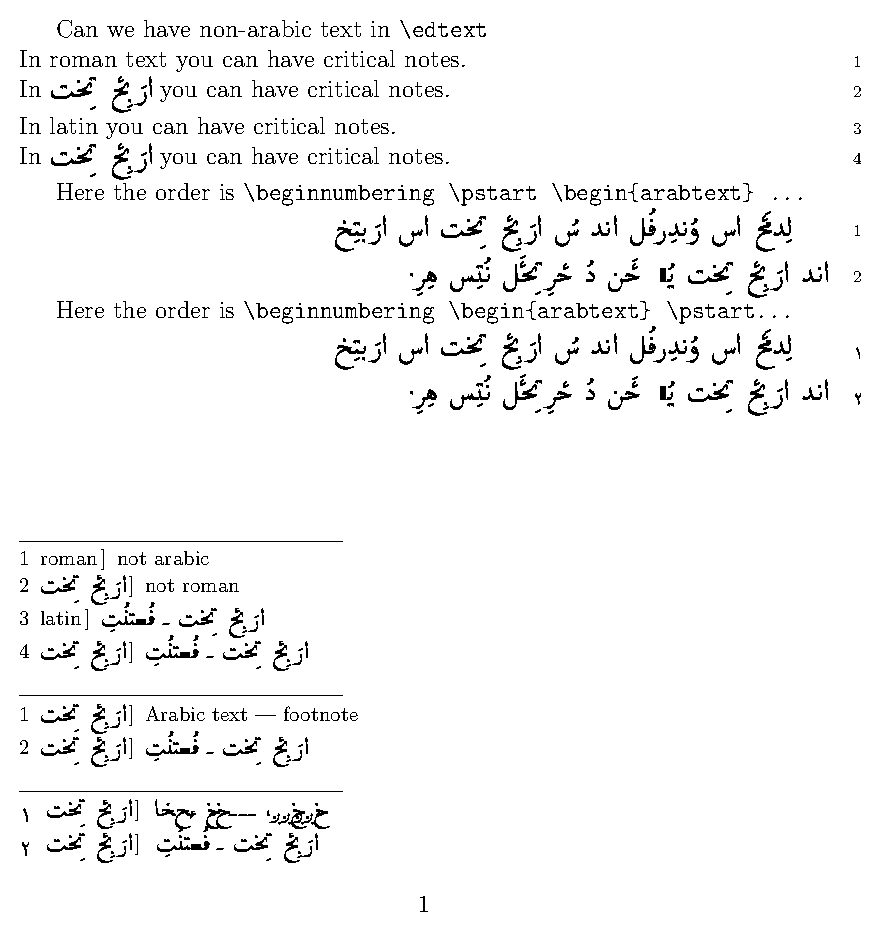
\includegraphics{egarab}
% \caption{Output from \texttt{egarab.tex}} \label{egarab-out}
% \end{addtomargins}
% \end{figure}
%
% \begin{figure}
% \begin{addtomargins}{-2cm}{-2cm}
% \centering
% 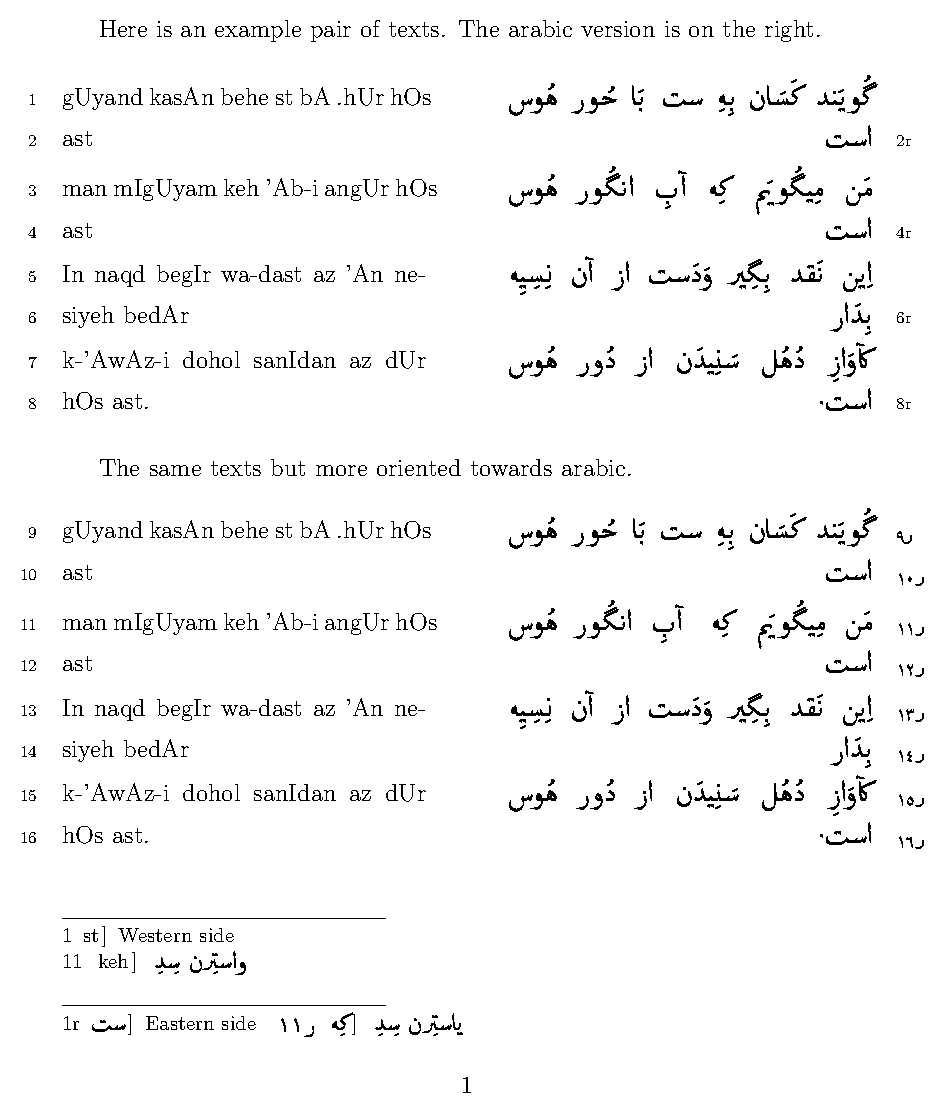
\includegraphics{egarabpar}
% \caption{Output from \texttt{egarabpar.tex}} \label{egarabpar-out}
% \end{addtomargins}
% \end{figure}
%
% \clearpage
%
% \subsection{General example}
%
% The result of the following code is shown in Figure~\ref{egarab-out}.
% The arabic script is nonsensical to anyone who can read Arabic
% as it is just the English text represented using the arabic script.
%
% The example illustrates a variety of critical notes, including one
% that is all messed up just to show that some things do not work.
%
% \medskip
% \hrule
% \medskip
%
%    \begin{macrocode}
%<*egarab>
%%% egarab.tex
\documentclass[12pt]{article}
\addtolength{\textheight}{-10\baselineskip}
\usepackage{ledmac}
\setcounter{firstlinenum}{1} \setcounter{linenumincrement}{1}
\linenummargin{right}

\usepackage{arabtex}
\usepackage{ledarab} 

\begin{document}

Can we have non-arabic text in \verb?\edtext?

\beginnumbering
\pstart
\noindent
In \edtext{roman}{\Afootnote{not arabic}} text you
can have critical notes. \\
In \edtext{\RL{Arabic text}}{\Afootnote{not roman}} you 
can have critical notes. \\
In \edtext{latin}{\Afootnote{\RL{Arabic text --- footnote}}} you 
can have critical notes. \\
In \edtext{\RL{Arabic text}}{\Afootnote{\RL{Arabic text --- footnote}}} you 
can have critical notes.
\pend
\endnumbering

Here the order is \verb?\beginnumbering \pstart \begin{arabtext} ...?

\beginnumbering
\pstart
\begin{arabtext}
ledmac is wonderful and so
%%% arabic lemma, latin note
\edtext{Arabic text}{\Bfootnote{Arabic text --- footnote}} is arabtex\\
%%% arabic lemma, arabic note
and \edtext{Arabic text}{\Bfootnote{\RL{Arabic text --- footnote}}} you 
can do critical notes here.
\end{arabtext}
\pend
\endnumbering

Here the order is \verb?\beginnumbering \begin{arabtext} \pstart...?

\arablnumrep
\beginnumbering
\begin{arabtext}
\pstart
ledmac is wonderful and so 
%%% arabic lemma, screwed up arabic note
\edtext{Arabic text}{\Cfootnote{Arabic text --- footnote}} is arabtex\\
%%% arabic lemma, arabic note
and \edtext{Arabic text}{\Cfootnote{\RL{Arabic text --- footnote}}} you 
can do critical notes here.
\pend
\end{arabtext}
\endnumbering
\restorelnumrep

\end{document}
%</egarab>
%    \end{macrocode}
%
% \subsection{Parallel example}
%
% The result of the following code for parallel typesetting is shown 
% in Figure~\ref{egarabpar-out}.
% The left and right inputs are the same. In this case the arabic script
% should make sense to an Arabic reader while the English text is the
% input that would produceds the arabic if it were inside the \texttt{arabtex}
% environment. The text for the example is from \file{omar.tex} in the
% \ArabTeX{} distribution; I do not know what it means.
%
% The two examples are virtually the same except that in the second the
% numbering is in arabic script instead of latin script. Note that 
% the usual variety of footnotes can be used for arabic texts as well 
% as western texts.
% 
% \medskip
% \hrule
% \medskip
%
%    \begin{macrocode}
%<*egarabpar>
%%% egarabpar.tex  ledmac & parallel arabic text
\documentclass[12pt]{article}
\addtolength{\textheight}{-4\baselineskip}
\usepackage{ledmac}
\usepackage{ledpar}
\setcounter{firstlinenum}{1} \setcounter{linenumincrement}{1}
\usepackage{arabtex}
\usepackage{ledarab}
%%
% simple right text arabic script numbering version of \printlines
\makeatletter
\def\printlinesAR#1|#2|#3|#4|#5|#6|#7|{\begingroup
  \setprintlines{#1}{#2}{#3}{#4}{#5}{#6}%
  \ifl@d@pnum #1\fullstop\fi
  \ifledplinenum \RL{#2}\Rlineflag\else \symplinenum\fi
  \endgroup}
\makeatother

%%% We will use the Bfootnote series for the arabic right texts,
%%% in paragraph style
\footparagraph{B}

%%% right text numbering 
\let\oldBfootfmt\Bfootfmt
\renewcommand{\Bfootfmt}[3]{%
  \let\printlines\printlinesR
  \oldBfootfmt{#1}{#2}{#3}}

\begin{document}

Here is an example pair of texts. The arabic version is on the right.

\vspace{\baselineskip}

\begin{pairs}

\begin{Leftside}
\beginnumbering
\pstart
\noindent 
gUyand kasAn behe \edtext{st}{\Afootnote{Western side}} bA .hUr  hOs ast \\
man mIgUyam keh 'Ab-i angUr hOs ast \\
In naqd begIr wa-dast az 'An nesiyeh bedAr \\
k-'AwAz-i dohol sanIdan az dUr hOs ast.
\pend
\end{Leftside}

\renewcommand{\Rlineflag}{r} % writes r in latin
\begin{Rightside}
\firstlinenum{2} \linenumincrement{2}
\begin{arabtext}
\beginnumbering
\pstart
\noindent 
gUyand kasAn behe \edtext{st}{\Bfootnote{Eastern side}} bA .hUr  hOs ast \\
man mIgUyam keh 'Ab-i angUr hOs ast \\
In naqd begIr wa-dast az 'An nesiyeh bedAr \\
k-'AwAz-i dohol sanIdan az dUr hOs ast. 
\pend
\end{arabtext}
\end{Rightside}

\Columns

\end{pairs}

\vspace{\baselineskip}

The same texts but more oriented towards arabic.

\vspace{\baselineskip}

\begin{pairs}

\begin{Leftside}
\pstart
\noindent 
gUyand kasAn behe st bA .hUr  hOs ast \\
man mIgUyam \edtext{keh}{\Afootnote{\RL{Western side}}} 'Ab-i angUr hOs ast \\
In naqd begIr wa-dast az 'An nesiyeh bedAr \\
k-'AwAz-i dohol sanIdan az dUr hOs ast.
\pend
\endnumbering
\end{Leftside}

%%% right full arabic note numbering
\renewcommand{\Bfootfmt}[3]{%
  \let\printlines\printlinesAR
  \oldBfootfmt{#1}{#2}{#3}}
\renewcommand{\Rlineflag}{\RL{r}} % writes r in arabic

\begin{Rightside}
\firstlinenum{1} \linenumincrement{1}
\arablnumrepR % changes the number to arabic
\begin{arabtext}
\pstart
\noindent 
gUyand kasAn behe st bA .hUr  hOs ast \\
man mIgUyam \edtext{keh}{\Bfootnote{\RL{Eastern side}}} 'Ab-i angUr hOs ast \\
In naqd begIr wa-dast az 'An nesiyeh bedAr \\
k-'AwAz-i dohol sanIdan az dUr hOs ast. 
\pend
\endnumbering
\end{arabtext}
\end{Rightside}

\begin{arabtext}
\Columns
\end{arabtext}

\end{pairs}

\end{document}
%</egarabpar>
%    \end{macrocode}
%
% 
%
% \bibliographystyle{alpha}
% \begin{thebibliography}{WWW99}
% \raggedright
%
% \bibitem[Lag99]{ARABTEX}
% Klaus Lagally.
% \newblock \emph{ArabTeX: A system for typesetting arabic: Draft User Manual},
% \newblock July 1999.
% \newblock (Available from CTAN in
%            \texttt{macros/latex/contrib/arabtex})
%
%
% \bibitem[LW90]{EDMACTUG}
% John Lavagnino and Dominik Wujastyk.
% \newblock `An overview of \edmac: a \textsc{Plain} TeX format for
%            critical editions'.
% \newblock \emph{TUGboat}, \textbf{11}, 4, pp. 623--643, November 1990.
% \newblock (Code available from CTAN in
%            \texttt{macros/plain/contrib/edmac})
%
%
% \bibitem[Wil04a]{LEDMAC}
% Peter Wilson.
% \newblock \emph{\Lpack{ledmac}: A presumptuous attempt to port \Lpack{EDMAC},
%                 \Lpack{TABMAC} and \Lpack{EDSTANZA} to LaTeX}.
% \newblock May 2004.
% \newblock (Available from CTAN in
%            \texttt{macros/latex/contrib/ledmac})
%
% \bibitem[Wil04b]{LEDPAR}
% Peter Wilson.
% \newblock \emph{Parallel typesetting for critical editions: 
%                 the \Lpack{ledpar} package}.
% \newblock December 2004.
% \newblock (Available from CTAN in
%            \texttt{macros/latex/contrib/ledmac})
%
% \end{thebibliography}
%
% \Finale
%
% \PrintIndex
% \endinput
\endinput

%% \CharacterTable
%%  {Upper-case    \A\B\C\D\E\F\G\H\I\J\K\L\M\N\O\P\Q\R\S\T\U\V\W\X\Y\Z
%%   Lower-case    \a\b\c\d\e\f\g\h\i\j\k\l\m\n\o\p\q\r\s\t\u\v\w\x\y\z
%%   Digits        \0\1\2\3\4\5\6\7\8\9
%%   Exclamation   \!     Double quote  \"     Hash (number) \#
%%   Dollar        \$     Percent       \%     Ampersand     \&
%%   Acute accent  \'     Left paren    \(     Right paren   \)
%%   Asterisk      \*     Plus          \+     Comma         \,
%%   Minus         \-     Point         \.     Solidus       \/
%%   Colon         \:     Semicolon     \;     Less than     \<
%%   Equals        \=     Greater than  \>     Question mark \?
%%   Commercial at \@     Left bracket  \[     Backslash     \\
%%   Right bracket \]     Circumflex    \^     Underscore    \_
%%   Grave accent  \`     Left brace    \{     Vertical bar  \|
%%   Right brace   \}     Tilde         \~}
%%
